\begin{frame}
  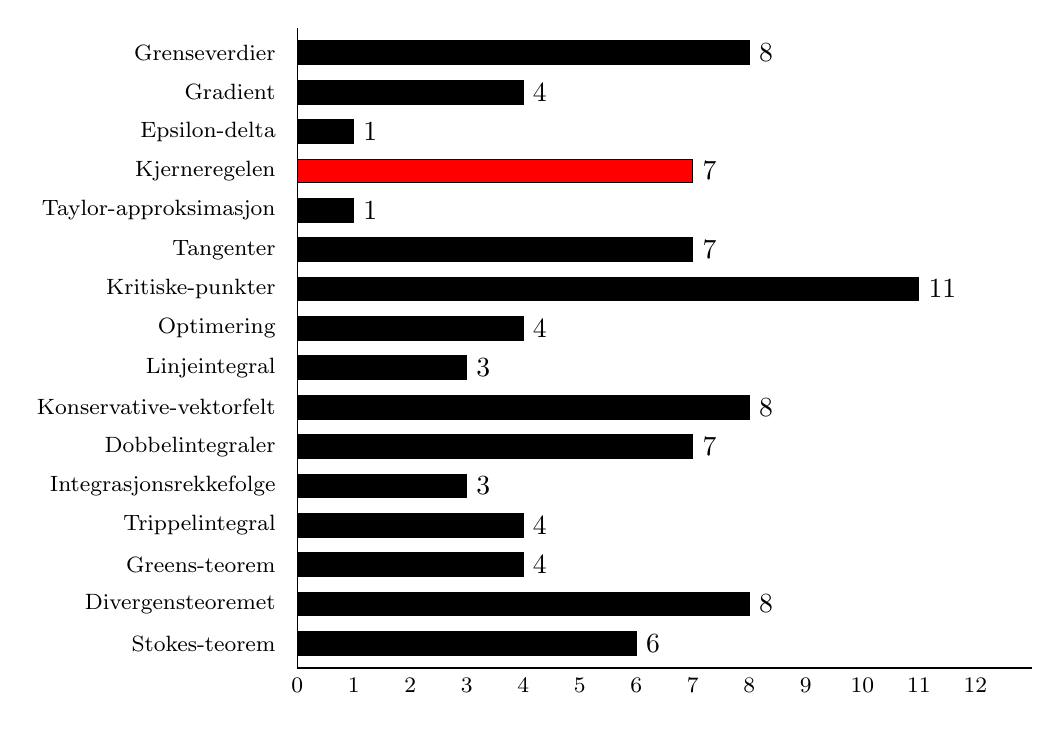
\begin{tikzpicture}
    \begin{axis}[ xbar=0pt, /pgf/bar shift=0pt, legend style={ legend columns=4,
        at={(xticklabel cs:0.5)}, anchor=north, draw=none }, ytick={0,...,15},
      ytick style={draw=none},% <- added
      axis y line*=none, axis x line*=bottom, tick label
      style={font=\footnotesize}, legend style={font=\footnotesize}, label
      style={font=\footnotesize}, xtick style={draw=none},% <- added
      xtick={0,1,...,12}, width=.9\textwidth, bar width=3mm, y dir = reverse,
      xmin=0, xmax=13, area legend,
      y=5mm, enlarge y limits={abs=0.625},
      style={text=black}, every axis plot/.append style={fill},
      nodes near coords, nodes near coords,
      yticklabels={%
        {\topicref{Grenseverdier}},
        {\topicref{Gradient}},
        {\topicref{Epsilon-delta}},
        {\topicref{Kjerneregelen}},
        {\topicref{Taylor-approksimasjon}},
        {\topicref{Tangenter}},
        {\topicref{Kritiske-punkter}},
        {\topicref{Optimering}},
        {\topicref{Linjeintegral}},
        {\topicref{Konservative-vektorfelt}},
        {\topicref{Dobbelintegraler}},
        {\topicref{Integrasjonsrekkefolge}},
        {\topicref{Trippelintegral}},
        {\topicref{Greens-teorem}},
        {\topicref{Divergensteoremet}},
        {\topicref{Stokes-teorem}}}]
      \addplot[fill=black] coordinates {(8,0)};
      \addplot[fill=black] coordinates {(4,1)};
      \addplot[fill=black] coordinates {(1,2)};
      \addplot[fill=red] coordinates {(7,3)};
      \addplot[fill=black] coordinates {(1,4)};
      \addplot[fill=black] coordinates {(7,5)};
      \addplot[fill=black] coordinates {(11,6)};
      \addplot[fill=black] coordinates {(4,7)};
      \addplot[fill=black] coordinates {(3,8)};
      \addplot[fill=black] coordinates {(8,9)};
      \addplot[fill=black] coordinates {(7,10)};
      \addplot[fill=black] coordinates {(3,11)};
      \addplot[fill=black] coordinates {(4,12)};
      \addplot[fill=black] coordinates {(4,13)};
      \addplot[fill=black] coordinates {(8,14)};
      \addplot[fill=black] coordinates {(6,15)};
    \end{axis}
  \end{tikzpicture}
\end{frame}

\begin{frame}
  \subsection{Kjerneregelen}\label{subsec:Kjerneregelen}
  \frametitle{Kjerneregelen}
  Anta vi skal derivere følgende funksjon
  %
  \begin{equation*}
    f(x,y) = \sin(x^2 - y^2) + \cos(y^2 - x^2)
  \end{equation*}
  %
  og ønsker å regne ut $x\tfrac{\partial f}{\partial y}+y\tfrac{\partial
    f}{\partial x}$.
  %
  \begin{align*}
    \diffp{f}{x}
    \only<1>{& = \diffp{}{x} \left( \sin(x^2 - y^2) \right) + \diffp{}{x}\left( \cos(y^2 - y^2) \right)\\}
    \only<2>{& = \diffp{}{x} \left( x^2 - y^2\right) \cos(x^2+y^2) - \diffp{}{x}\left( y^2 - x^2) \right) \sin(y^2 - x^2)\\}
    \only<3>{& = \phantom{-}2x \cos(x^2+y^2) + 2x \sin(y^2 - x^2)\\}
      \diffp{f}{y}
    \only<1>{& = \diffp{}{y} \left( \sin(x^2 - y^2) \right) + \diffp{}{y}\left( \cos(y^2 - x^2) \right)\\}
    \only<2>{& = \diffp{}{y} \left( x^2 - y^2\right) \cos(x^2+y^2) - \diffp{}{y}\left( y^2 - x^2) \right) \sin(y^2 - x^2)\\}
    \only<3>{& = -2y \cos(x^2+y^2) - 2y \sin(x^2 - y^2)}
  \end{align*}
  \only<3>{Ved inspeksjon ser vi at $x\tfrac{\partial f}{\partial y}+y\tfrac{\partial
    f}{\partial x} = 0$. Men gjelder dette alltid?}
\end{frame}

\begin{frame}
  \begin{oppgave}{K2014, Oppgave 2}
    Gitt $z = f (x, y)$ der $f$ er en deriverbar funksjon og
    $x = u^2 - v^2$ , $y = v^2 - u^2$. Vis at
    %
    \begin{equation*}
      u \diffp{z}{v} + v \diffp{z}{u} = 0\,.
    \end{equation*}
  \end{oppgave}
  Bruker kjerneregelen på $z = f(x,y) = f(u^2 - v^2, v^2 - u^2)$.
  %
  \begin{align*}
    \diffp{z}{u}
    \only<1>{& = \diffp{}{u} \left( f(x(u,v), y(u,v)) \right) \\}
    \only<2>{& = \diffp{x}{u}\diffp{f}{x} + \diffp{y}{u}\diffp{f}{y}\\}
    \only<3>{& = \phantom{-}2u\diffp{f}{x} - 2u\diffp{f}{y}\\}
      \diffp{z}{v}
    \only<1>{& = \diffp{}{v} \left( f(x(u,v), y(u,v)) \right)\\}
    \only<2>{& = \diffp{x}{v}\diffp{f}{x} + \diffp{y}{v}\diffp{f}{y}\\}
    \only<3>{& = -2v\diffp{f}{x} + 2v\diffp{f}{y}}
  \end{align*}
  \only<3>{Ved inspeksjon ser vi at $u\tfrac{\partial f}{\partial v}+v\tfrac{\partial
    f}{\partial u} = 0$ for alle deriverbare funksjoner $z=f(x,y)$.}
\end{frame}



%%% Local Variables:
%%% mode: latex
%%% TeX-master: "main"
%%% End:
